\documentclass[10pt, compress]{beamer}

\usetheme{m}

\usepackage{booktabs}
\usepackage[scale=2]{ccicons}
\usepackage{minted}
\usepackage{hyperref}
\usepackage{xcolor}

\usemintedstyle{trac}

\title{Required Skills for Software Development}
\subtitle{}
\date{\today}
\author{Mohammad-Ali \textsc{A'r\^abi}}
\institute{Albert-Ludwigs-Universität Freiburg}

\begin{document}

\maketitle

\section{Programming Languages}

\begin{frame}[fragile]
    \frametitle{StackOverflow Survey 2019}
  
    \begin{table}[c]
        \centering
        \begin{tabular}{l|cc}
            Language & Pros & All \\
            \hline
            JavaScript & 1 & 1 \\
            Python & 2 & 2 \\
            Java & 3 & 3 \\
            C\# & 4 & 4 \\
            PHP & 5 & 5 \\
            TypeScript & 6 & 7 \\
            C++ & 7 & 6 \\
            C & 8 & 8 \\
            Ruby & 9 & 9 \\
            Go & 10 & 10
        \end{tabular}
        \caption{Top 10 programming languages}
        \label{tab:stackoverflow-top-10}
    \end{table}

\end{frame}

\begin{frame}[fragile]
    \frametitle{PyPL Index 2020}
    
    \begin{table}
        \centering
        \begin{tabular}{ll|l|ll}
            Rank & Change & Language & Share & Trend \\ \hline
            1 &  & Python & 31.17 \% & +4.3 \% \\ 
            2 &  & Java & 17.75 \% & -2.4 \% \\ 
            3 &  & Javascript & 7.99 \% & -0.3 \% \\ 
            4 &  & C\# & 7.05 \% & -0.2 \% \\ 
            5 &  & PHP & 6.09 \% & -1.0 \% \\ 
            6 &  & C/C++ & 5.67 \% & -0.3 \% \\ 
            7 &  & R & 3.93 \% & -0.1 \% \\ 
            8 &  & Objective-C & 2.4 \% & -0.4 \% \\ 
            9 &  & Swift & 2.26 \% & -0.1 \% \\ 
            10 & -1 & TypeScript & 1.89 \% & +0.3 \% \\
        \end{tabular}
        \caption{Top 10 programming languages}
        \label{tab:pypl-top-10}
\end{table}
\end{frame}

\begin{frame}[fragile]
    \frametitle{Octaverse}
    
    \begin{figure}
        \centering
        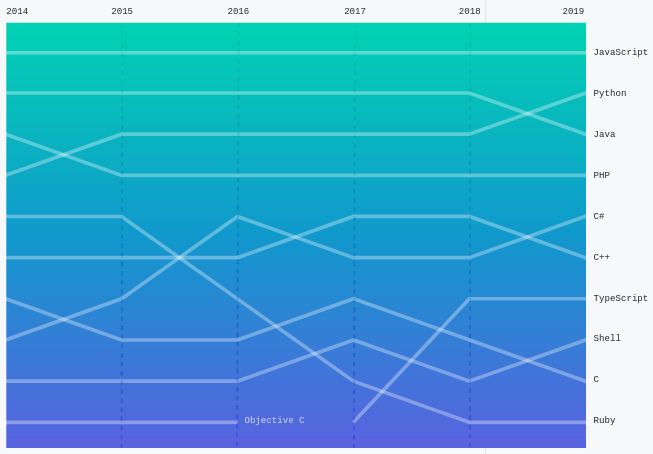
\includegraphics[scale=0.4]{images/octaverse.png}
        \caption{Top 10 programming languages}
        \label{fig:octaverse-top-10}
    \end{figure}
\end{frame}

\plain{}{Questions?}

\end{document}
